%!TEX root = alga.tex
\vspace{-2mm}
\section{Introduction}\label{sec-intro}
\vspace{-0.5mm}

Graphs are ubiquitous in computing, yet working with graphs often requires
painfully low-level fiddling with sets of vertices and edges. Building high-level
abstractions is difficult, because the commonly used foundation -- the pair $(V, E)$
of vertex set $V$ and edge set $E \subseteq V \times V$ -- is a source of partial
functions. We can represent the pair $(V, E)$ by the following simple data
type\footnote{Although in this paper we exclusively use Haskell, the problem we solve is
general and the proposed approach can be readily adapted to other programming languages.}:

\vspace{0.5mm}
\begin{minted}{haskell}
  data G a = G { vertices :: [a], edges :: [(a,a)] }
\end{minted}
\vspace{0.5mm}

\noindent
Now \hs{G@\,\,@[1,2,3]@\,\,@[(1,2),(2,3)]} is the graph with three vertices $V = \{1,2,3\}$ and
two edges $E = \{(1,2), (2,3)\}$. The consistency invariant $E \subseteq V \times V$ holds.
But what is \hs{G@\,\,@[1]@\,\,@[(1,2)]}? The edge refers to the non-existent vertex $2$, breaking the
invariant, and there is no easy way to reflect this in types. Perhaps, our data type is just
too simplistic; let us look at state-of-the-art graph libraries instead.

The \textsf{containers} library is designed for performance and powers GHC itself.
It represents graphs by \emph{adjacency arrays}~\cite{1995_king_graphs} whose
consistency invariant is not statically checked, which can lead to runtime
usage errors such as \textsf{`index out of range'}. Another popular library \textsf{fgl} uses
the \emph{inductive graph representation}~\cite{2001_erwig_inductive}, but its API also
has partial functions, e.g. inserting an edge can fail with the \textsf{`edge from
non-existent vertex'} error.
Both \textsf{containers} and \textsf{fgl} are treasure troves of graph algorithms,
but it is easy to make an error when using them. Is there a safe graph construction
interface we can build on top?

In this paper we present \emph{algebraic graphs} --- a new interface for constructing
and transforming graphs (more precisely, graphs with labelled vertices and unlabelled
edges). We abstract away from graph representation details and characterise graphs by a
set of axioms, much like numbers are algebraically characterised by
\emph{rings}~\cite{1999_maclane_algebra}. Our approach is based on the
\emph{algebra of parameterised graphs}, a mathematical formalism used in digital
circuit design~\cite{2014_algebra_mokhov}, which we simplify and adapt to the
context of functional programming.

Algebraic graphs have a safe and minimalistic core of four graph construction primitives,
as captured by the following data type:

\vspace{-0.59mm}
\begin{minted}{haskell}
  data Graph a = Empty
               | Vertex a
               | Overlay (Graph a) (Graph a)
               | Connect (Graph a) (Graph a)
\end{minted}
\vspace{-0.59mm}

\noindent
Here \hs{Empty} and \hs{Vertex} construct the \emph{empty} and \emph{single-vertex} graphs,
respectively; \hs{Overlay} composes two graphs by taking the union of their vertices and
edges, and \hs{Connect} is similar to \hs{Overlay} but also creates edges between vertices
of the two graphs, see~Fig.~\ref{fig-construction} for examples. The \emph{overlay} and
\emph{connect} operations have two important properties:
(i) they are closed on the set of graphs, i.e. are total functions, and (ii) they can be used
to construct any graph starting from the empty and single-vertex graphs.
For example, \hs{Connect@\,\,@(Vertex@\,\,@1)@\,\,@(Vertex@\,\,@2)} is the graph with two vertices $\{1,2\}$
and a single edge $(1,2)$. Malformed graphs, such as \hs{G@\,\,@[1]@\,\,@[(1,2)]}, cannot be
expressed in this core language.

The main goal of this paper is to demonstrate that \emph{this core is a safe, flexible
and elegant foundation for working with graphs that have no edge labels}. Our specific
contributions are:
\vspace{-0.25mm}
\begin{itemize}
  \item Compared to existing libraries, algebraic graphs have a smaller
  core (just four graph construction primitives), are more compositional
  (hence greater code reuse), and have no partial functions (hence fewer
  opportunities for usage errors). We present the core and justify these claims
  in \S\ref{sec-core}.

  \item The core has a simple mathematical structure fully characterised
  by a set of axioms~(\S\ref{sec-algebra}). This makes the
  proposed interface easier for testing and formal verification. We show that
  the core is \emph{complete}, i.e. any graph can be constructed, and \emph{sound},
  i.e. malformed graphs cannot be constructed.

  \item Under the basic set of axioms, algebraic graphs correspond to directed
  graphs. As we show in~\S\ref{sec-a-la-carte}, by extending
  the algebra with additional axioms, we can represent undirected,
  reflexive, transitive graphs, their combinations, and hypergraphs.
  Importantly, the core remains unchanged, which allows us to define highly
  reusable polymorphic functions on graphs.

  \item We develop a library\footnote{The library is on Hackage:
  \url{http://hackage.haskell.org/package/algebraic-graphs}.}
  for constructing and transforming algebraic graphs
  and demonstrate its flexibility in \S\ref{sec-transformations}.

  % Although the development of efficient algorithms for algebraic
  % graphs is outside the scope of this paper, we show that the library can cope
  % with graphs comprising billions of edges in the matter of
  % seconds, which is sufficiently fast for many applications.
\end{itemize}
\vspace{-2mm}

\begin{figure*}
\begin{subfigure}[b]{0.2\linewidth}
\centerline{
\includegraphics[scale=0.27]{fig/ex-a.pdf}}
\vspace{-2.4mm}
\caption{$1 + 2$}
\centerline{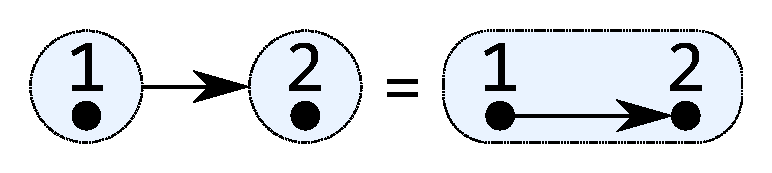
\includegraphics[scale=0.27]{fig/ex-b.pdf}}
\vspace{-2.4mm}
\caption{$1 \rightarrow 2$}
\end{subfigure}
\hspace{11mm}
\begin{subfigure}[b]{0.17\linewidth}
\centerline{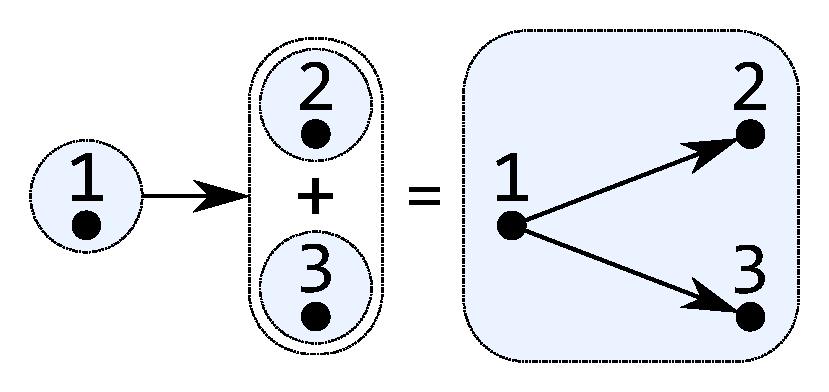
\includegraphics[scale=0.27]{fig/ex-c.pdf}}
\vspace{-1mm}
\caption{$1 \rightarrow (2 + 3)$}
\end{subfigure}
\hspace{12mm}
\begin{subfigure}[b]{0.15\linewidth}
\centerline{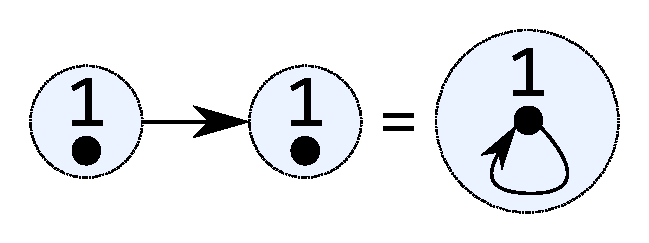
\includegraphics[scale=0.27]{fig/ex-d.pdf}}
\vspace{2.4mm}
\caption{$1 \rightarrow 1$}
\end{subfigure}
\hspace{12mm}
\begin{subfigure}[b]{0.2\linewidth}
\centerline{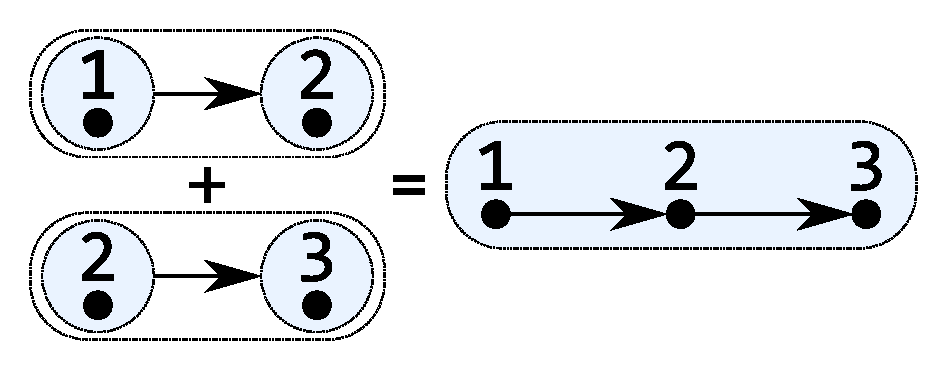
\includegraphics[scale=0.27]{fig/ex-e-new.pdf}}
\vspace{-1mm}
\caption{$1 \rightarrow 2 + 2 \rightarrow 3$}
\end{subfigure}
\vspace{-1.5mm}
\caption{Examples of graph construction. The overlay and connect operations are denoted
by $+$ and $\rightarrow$, respectively.\label{fig-construction}}
\vspace{-3mm}
\end{figure*}

Graphs and functional programming have a long history. We review related
work in \S\ref{sec-related}. Limitations of the presented approach and future
research directions are discussed in \S\ref{sec-discussion}.
